% 4.3 O3 Economy, politics and society. OWNER: Prerna. First draft by Aryan from the deck (slides 30-31) and the D3
% country table (report/analysis/d3_country_table.py). Numbers: claims.csv rows O3, S5/O3; claims_report.csv.
\subsection{O3: Economy, politics and society}\label{sec:o3}

\begin{table*}[t]\centering
\caption{Country table (deliverable D3): the 12 countries with a tracked AI site. MW: facility power today and planned
by the end of 2030. Population: GHSL 2025 (world: 8.19 billion). $LQ$: share of capacity $\div$ share of world
population (``--'': no capacity yet). Stressed: share of the country's planned MW in basins of high or extremely high
baseline stress. People: within 50\,km of any of the country's sites, counted once; Malaysia's Johor sites include
residents of Singapore. Water: our low--high consumption range for the planned capacity, direct plus indirect.
Country-level Gini of capacity per person: 0.936 today, 0.940 for the 2030 plan.}
\label{tab:d3}
\footnotesize\renewcommand{\arraystretch}{1.08}\setlength{\tabcolsep}{3.7pt}
\begin{tabular}{@{}l r r r r r r r r r r r@{}}
\toprule
 & & \multicolumn{2}{c}{MW} & Share of & Population & \multicolumn{2}{c}{$LQ$} & W per person & Stressed & People
 & Water 2030 \\
\cmidrule(lr){3-4}\cmidrule(lr){7-8}
Country & Sites & today & 2030 & 2030 MW (\%) & (M) & today & 2030 & (2030) & (\% of MW) & $\le$50\,km (M) & (bn L/yr) \\
\midrule
\tabin{tables/d3_country.tex}
\bottomrule
\end{tabular}
\end{table*}

\paragraph{Capacity is far more concentrated than people} The United States holds 83.4\% of the 15,078\,MW tracked
today and 86.2\% of the 2030 plan, with 4.2\% of the world's population (\Tab{tab:d3}). Its location quotient is
therefore about 20: twenty times its population share. Malaysia, with several large sites in Johor next to Singapore,
has almost the same quotient today (19.5), falling to 9.2 by 2030 as US capacity grows faster. The highest 2030 quotient
belongs to the United Arab Emirates (24.0), where one planned 1.4\,GW campus serves 9.5 million residents. The Nordic
countries and Iceland sit between 4 and 8, reflecting a few sites in small populations. At the other end, China hosts
5.9\% of today's tracked capacity with 17.4\% of the world's people ($LQ$ 0.34) and Indonesia 0.5\% with 3.4\% (0.14).
The 2030 plan works out at 127\,W per person in the United States against a world average of 6.1\,W, and 73\% of
the world's people live in countries with no tracked AI site at all.

\begin{figure}[t]\centering
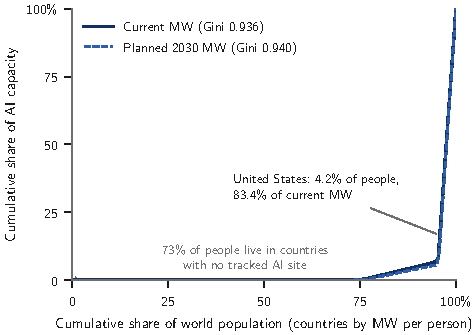
\includegraphics[width=\linewidth]{figs/o3_lorenz.pdf}
\caption{Lorenz curve of tracked AI capacity against population, by country (deliverable D3). Countries are sorted
by MW per person; the diagonal would be perfect equality. Countries without a tracked site are pooled at zero, which
leaves the Gini unchanged.}
\label{fig:lorenz}
\end{figure}

\paragraph{The country-level Gini} The Lorenz curve (\Fig{fig:lorenz}) hugs the bottom axis until the last few
percent of the world's population. The Gini coefficient of capacity per person is 0.936 for current capacity and 0.940
for the 2030 plan. The presented deck reported 0.927 from seven country groups (with UN population data,
\citealp{undesa2024}); pooling
countries inside groups hides inequality within them, so the group value is a lower bound, and the country-level value
is indeed higher. Among the host countries alone the Gini is 0.76 (0.78 for 2030): even among countries that host AI
capacity, it is very unevenly spread. Both values describe the Epoch sample, which is AI-only and US-heavy (Section
\ref{sec:limits}); they measure where large AI campuses are being built, not all digital infrastructure.

\paragraph{Water stress and exposure by country} The country view also shows where the water pressure of
Section~\ref{sec:o2} lands. In the United States 39\% of the planned capacity is in stressed basins, and 68 million
people live within 50\,km of a site. China's share is 24\%; Malaysia's sites are all in lower-stress basins. Four
countries (the UAE, Portugal, the United Kingdom and Australia) have a single site each, all in stressed basins, so
their 100\% is one site, not a pattern.

\paragraph{Local opposition is rising} In the United States, organised opposition is now common. Data Center Watch
counts at least 75 projects worth about US\$130 billion blocked or delayed in the first quarter of 2026, with the
number of active opposition groups more than doubled since the end of 2025 and present in 49 states \citep{dcw2026}.
The second quarter eased but stayed high: at least 45 projects worth about US\$68 billion, and 843 opposition groups, up from 833
at the end of March \citep{dcw2026q2}.
We code disputes with five grievance tags adapted from the EJAtlas \citep{temper2015}: \emph{water} (cooling
withdrawals, basin stress, competition with households and farms), \emph{power} (grid connection, new generation,
electricity bills, fossil lock-in), \emph{noise} (fans, chillers, backup generators), \emph{land} (campus footprint,
rezoning, habitat) and \emph{jobs} (construction against permanent jobs). This is a coding framework, not a measured
total; both of our case studies are water disputes. Supply-chain concentration, the third part of O3, is shown in
\Fig{fig:materials}: the minerals come from a few countries, and one export ban can reach the whole build-out.

\begin{finding}{Finding 5. Capacity per person is twenty times the world share in the US and Malaysia}
Country-level Gini 0.94: 73\% of the world's people live in countries with no tracked AI site. The concentration that
makes AI's footprint small globally is what makes it large locally.
\end{finding}
